\documentclass[../Cours.tex]{subfiles}

\usepackage{xstring}
\usepackage{xfp}

\begin{document}
\clearpage
\thispagestyle{empty}

\color{black}
\nomPrenom
\titreDS

\begin{questions}
    \EXERCICETITRE{3}{Nombres relatifs}
    \question Classer ces évènements \textit{du plus ancien au plus récent}.
        \begin{multicols}{2}
        \subquestion Sacrement de Napoléon : 1804
        \subquestion Chute de l'Empire romain : 476
        \subquestion Naissance de Toutânkhamon : -1345
        \subquestion Naissance de Jules César : -100
        \subquestion Sacrement de Louis IX : 1214
        \subquestion Naissance de Cléopâtre VII : -69
        \end{multicols} 
    \caseReponse{1.5}
    \question Classer ces éléments dans \textit{l'ordre croissant} de leur température de fusion.
        \begin{multicols}{3}
        \subquestion Fer : \qty{1538}{\degreeCelsius}
        \subquestion Eau : \qty{0}{\degreeCelsius}
        \subquestion Diazote : \qty{-210.01}{\degreeCelsius}
        \subquestion Or : \qty{1064.18}{\degreeCelsius}
        \subquestion Ozone : \qty{-192.5}{\degreeCelsius}
        \subquestion Chocolat : \qty{45}{\degreeCelsius}
        \end{multicols}
    \caseReponse{1.5}

    \EXERCICETITRE{4}{Parallélogrammes}
    \question Donner et justifier la nature de ce quadrilatère.

    \begin{centre}
        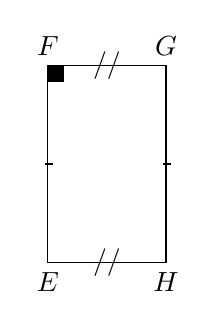
\begin{tikzpicture}
            %\draw (0,0) node[below]{$A$} -- +(1,2) node[left]{$B$}  node[midway]{\_}-- +(4,2) node[right]{$C$}  node[midway]{//}-- +(3,0) node[below]{$D$}  node[midway]{\_}-- cycle node[midway]{//};
            \draw (6,0) node[below]{$E$} -- +(0,2.5) node[above]{$F$} node[midway]{\_} -- +(1.5,2.5) node[above]{$G$} node[midway]{//} -- +(1.5,0) node[below]{$H$} node[midway]{\_} -- cycle node[midway]{//};
            \filldraw (6,2.5) rectangle +(0.2,-0.2);
            %\draw (9,1) node[left]{$I$} -- +(1,1.4) node[above]{$J$} node[midway]{\textbackslash} -- +(2,0) node[right]{$K$} node[midway]{/} -- +(1,-1.4) node[below]{$L$} node[midway]{\textbackslash} -- cycle node[midway]{/};
        \end{tikzpicture}
    \end{centre}    
    \caseReponse{6}

    \EXERCICETITRE{4}{Alcool au volant}
    D'après l'article R234-1 du code de la route : <<  Même en l'absence de tout signe d'ivresse manifeste, est puni de l'amende prévue pour les contraventions de la quatrième classe le fait de conduire un véhicule sous l'empire d'un état alcoolique caractérisé par : [...] \textbf{Une concentration d'alcool dans le sang égale ou supérieure à 0,50 gramme par litre}. >> 
    \question Si on prélève à un conducteur \qty{5}{\milli\litre} de sang, et qu'il contient \qty{2}{\milli\gram} d'alcool, a-t-on le droit de conduire ?
    \caseReponse{3}
    \question Supposons qu'un adulte possède \qty{6}{\litre} de sang dans son corps. S'il a une concentration en alcool dans le sang de \qty{0.50}{\gram\per\litre}, quelle sera la quantité totale d'alcool dans son corps ?
    \caseReponse{3}
    \question Pour la prise de sang, on utilise une seringue. Elle a la forme d'un cylindre de rayon \qty{7.22}{\milli\metre} et de hauteur \qty{85.48}{\milli\metre}. 
    \subquestion Quel est son volume ? (rappel : $V_{\mbox{cylindre}} = \pi r^2 h$)
    \caseReponse{3}
    \subquestion Est-elle suffisante pour la prise de sang de \qty{5}{\milli\litre} ?
    \caseReponse{3}

    \clearpage
    \EXERCICETITRE{7}{Diagrammes}
    On s'intéresse aux émissions de gaz à effet de serre en France, par année et par secteur d'activité. Le premier tableau ci-dessous donne les émissions de gaz à effet de serre en France entre 1990 et 2020 :
    \begin{center}
        \begin{flushright}
            \textit{En millions de tonnes équivalent $CO_2$}
        \end{flushright}
        \begin{tabularx}{0.8\linewidth}{|l|X|X|X|X|X|X|X|}\hline
            Année & 1990 & 1995 & 2000 & 2005 & 2010 & 2015 & 2020  \\\hline
            Émission & \num{544.1} & \num{536.5} & \num{549.0} & \num{551.4} & \num{507.5} & \num{457.9} & \num{393.0} \\\hline
        \end{tabularx}
        \begin{flushright}\vspace{-0.8em}
            \textit{(source INSEE)}
        \end{flushright}
    \end{center}

    \question Compléter le diagramme en barres ci-dessous : 
    \begin{center}
        \begin{tikzpicture}[xscale=1.2,yscale=0.8]
            \draw[-Latex] (0,0) -- (12,0);
            \draw[-Latex] (0,0) -- (0,7);
            \foreach \x in {1.5,3,...,10.5} {
                \draw (\x,-0.2) -- (\x,0.2);
                \node[below] at (\x,-0.2) {\pgfmathparse{int(int(\x*2/3)*5+1985)}\pgfmathresult};
            }
            \foreach \y in {0,1,...,6} {
                \draw[gray] (0,\y) -- (12,\y);
                \node[left] at (0,\y) {\small{\y}};
            }
            \foreach \i in {0,1,...,5} {
                \foreach \y in {0.2,0.4,0.6,0.8} {
                    \draw[gray!40!white] (0,{\i+\y}) -- +(12,0);
                }
            }
            \filldraw (1.2,0) rectangle (1.8,5.441);
        \end{tikzpicture}
    \end{center}

    On s'intéresse maintenant à la répartition des émissions de gaz à effet de serre par secteur d'activité pour l'année 2021 en France : 
    \begin{center}
        \begin{flushright}
            \textit{En millions de tonnes équivalent $CO_2$}
        \end{flushright}
        \begin{tabularx}{0.8\linewidth}{|l|X|X|}\hline
        Secteur d'activité & Émission & Degrés \\\hline\hline
        Industrie de l’énergie & \num{43.1} &  \\\hline
        Industrie manufacturière et construction & \num{77.8} &  \\\hline
        Traitement centralisé des déchets & \num{14.5} &  \\\hline
        Usage des bâtiments et activités résidentiels/tertiaires & \num{74.9} &  \\\hline
        Agriculture/sylviculture & \num{81.2} &  \\\hline
        Transport routier & \num{119.6} & \\\hline
        Autres transports & \num{6.4} &  \\\hline\hline
        Ensemble & \num{418.2} & \textbf{\ang{360}} \\\hline
        \end{tabularx}
        \begin{flushright}\vspace{-0.8em}
            \textit{(source INSEE)}
        \end{flushright}
    \end{center}

    \question Compléter le tableau pour calculer les angles nécessaires au diagramme circulaire.
    \question Compléter le diagramme circulaire ci-dessous : 
    \begin{center}
        \begin{tikzpicture}[scale=0.9]
            \draw (0,0) circle (2.7);
            \draw (0,0) -- (2.7,0);
            \foreach \i in {1,...,7} {
                \draw (4,{2.5 - \i*0.7}) rectangle +(0.3,0.3);
                \draw (4.4,{2.5 - \i*0.7}) -- +(6,0);
            }
        \end{tikzpicture}
    \end{center}
\end{questions}
\end{document}